\documentclass{article}
\usepackage[utf8]{inputenc}
\usepackage{graphicx}
\usepackage[spanish,es-tabla]{babel}
\usepackage{amsmath}
\usepackage[a4paper,margin=1in,footskip=.5cm]{geometry}
\usepackage{subcaption}
\setlength\headheight{30pt} 
\usepackage{fancyhdr}
\usepackage{amssymb}
\usepackage[hidelinks]{hyperref}
\usepackage{mathtools}
\usepackage[table,xcdraw]{xcolor}
\usepackage[backend=bibtex]{biblatex}
\usepackage{csquotes}
\usepackage{float}
\hypersetup{
colorlinks = true,
urlcolor=blue,
linkcolor = black
}
\addbibresource{bibliography.bib} %archivo de bibliografia

\begin{document}



% agregamos la caratula
\begin{titlepage}
    

\thispagestyle{empty}

% Portada Custom, ver /maketitle: https://www.overleaf.com/learn/latex/How_to_Write_a_Thesis_in_LaTeX_(Part_5)%3A_Customising_Your_Title_Page_and_Abstract

\begin{center}
    
\includegraphics[width=5cm]{img/unc_logo.png} \hspace{2cm}
    
\includegraphics[width=5cm]{img/fcefyn_logo.jpg}
    \\[1cm]
    \vspace{5pt}
   \vspace{5pt}
    \LARGE Universidad Nacional de Córdoba\\[0.5cm] 
    \large Facultad de Ciencias Exactas, Físicas y Naturales \\[0.5cm] 
    \large Sintesis de Redes Activas
    \\[0.2cm]
    \large TP N° 1
    \\[0.2cm]
    \large A.O Ideal
    \\[0.2cm]
    \large Grupo 3
    \\[0.2cm]
    \vspace{60pt}
    \begin{table}[!h]
    \centering
    \begin{tabular}{ll}
    \multicolumn{1}{c}{Nombre} & \multicolumn{1}{c}{DNI} \\
    Cruz Enrique Luis & 42072368 \\
    Galvagno Facundo& 40815088 \\
    Yomaha Gaston & 43298118 \\
    Vega Guadalupe & 43233268 \\
    Zuñiga Guillermo Ruben & 44229491\\
    
    \end{tabular}
    \end{table}
    \vspace{20pt}
    \begin{table}[!h]
    \centering
    \begin{tabular}{ll}
    \multicolumn{1}{c}{Docentes} & Ing. César Reale \\
     & Ing. Pablo Ferreyra
    \end{tabular}
    \end{table}
    \vfill
    Córdoba, República Argentina\\
    \today
\end{center}

\end{titlepage}
\newpage

% agregamos el indice
\tableofcontents
\newpage



\section{Introducción}

En el presente informe se desarrolla el analisis teórico de cuatro circuitos diferentes: 

\begin{enumerate}
    \item Amplificador diferencial
    \item Fuente de corriente controlada por tensión
    \item Rectificador de precisión
    \item Comparador con histéresis
\end{enumerate}

Para contar con más comodidad a la hora de realizar mediciones, se utilizó Kicad para diseñar un PCB. El PCB se fabricó a modo de prototipo rápido.

\begin{figure}[H]
    \centering
    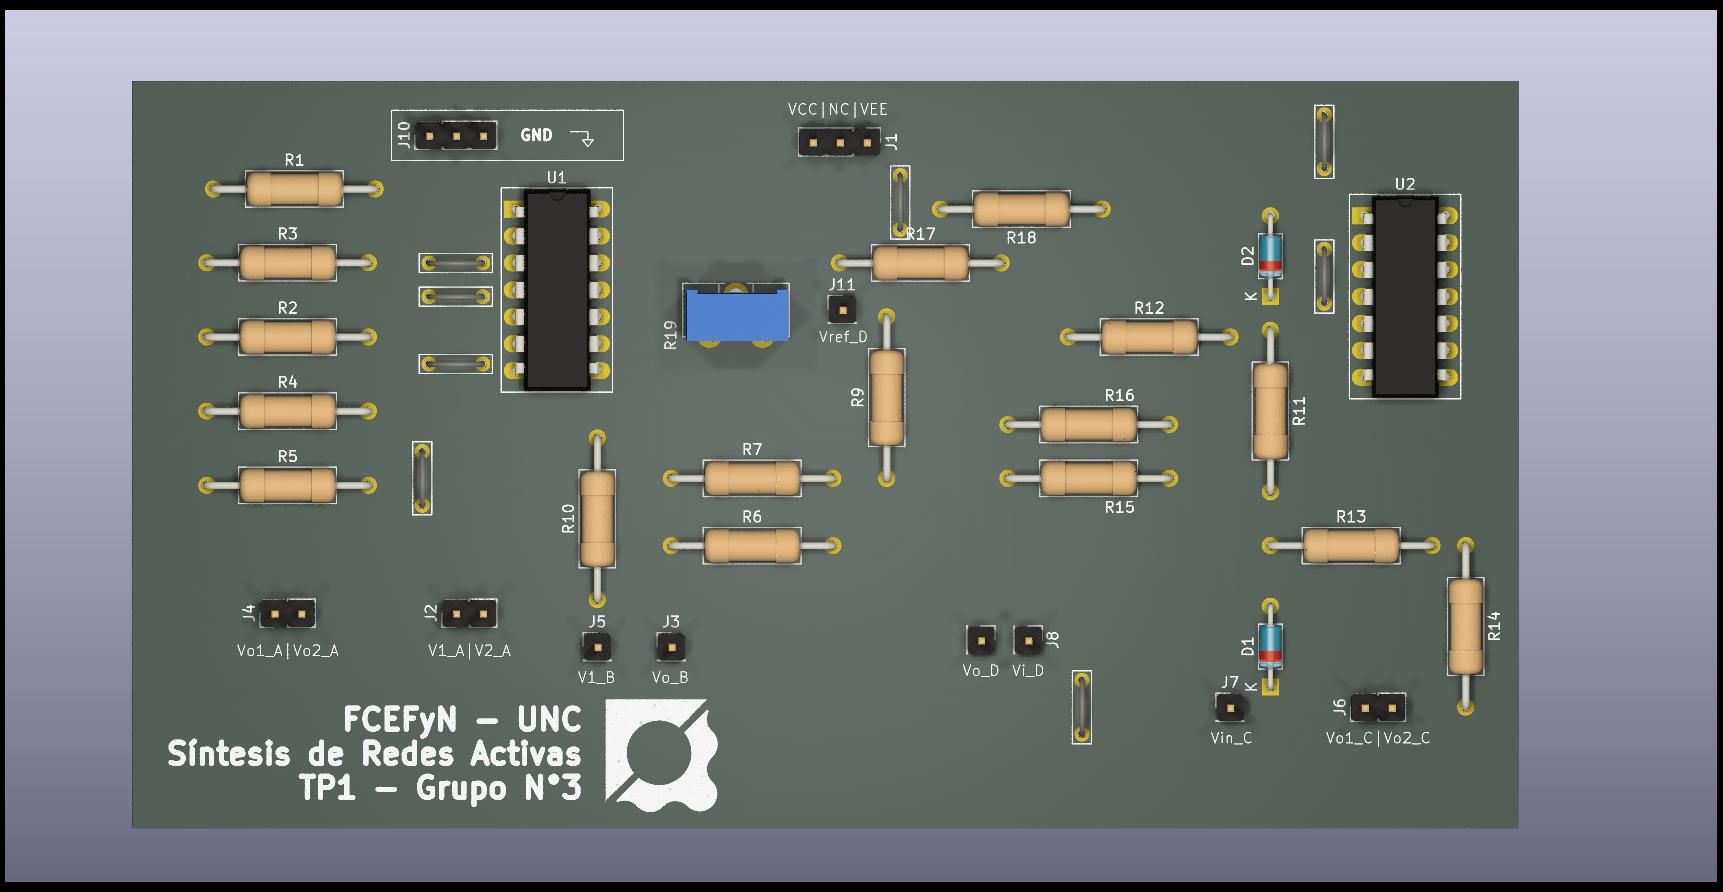
\includegraphics[width=1\linewidth]{LABN1_SRA.jpg}
    \caption{PCB utilizado para realizar mediciones}
    \label{fig:enter-label}
\end{figure}

%Analisis1
\section{Circuito n° 3: Rectificador de precisión }

\subsection{Análisis Teórico}

\begin{figure}[H]
    \centering
    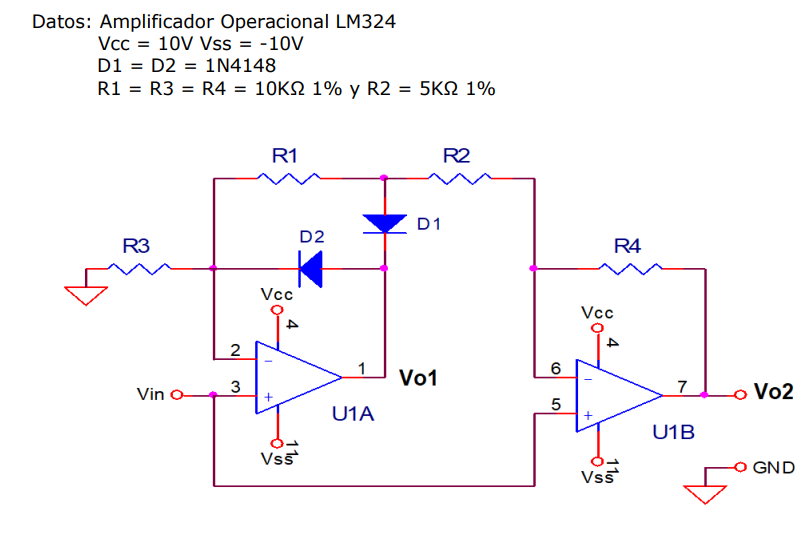
\includegraphics[width=0.5\linewidth]{Secciones/Circuito3/circuito.png}
    \caption{Circuito del rectificador}
    \label{fig:Circuito3}
\end{figure}

Para determinar la tensión de salida Vo en función de la tensión de entrada Vin, se considerarán dos casos: cuando la tensión de entrada es positiva, y cuando la tensión de entrada es negativa.

\[V_0 = f(V_{in}) \ \text{con} \ 0 < V_{in}\]

En estas condiciones, el diodo D2 conduce, mientras que el diodo D1 no, ya que el amplificador U1A se encuentra operando en modo no inversor.
Inicialmente se analizará el caso en que la tensión de entrada del amplificador U1B se encuentra pasivada, entonces la ecuación de corrientes en el nodo ‘6’ resulta:

\begin{equation}
\frac{V_o}{R_4} = \frac{V_in}{R_1 + R_2}
\end{equation}

\begin{equation}
\frac{V_o}{10[k\Omega]} = -\frac{V_{in}}{15[k\Omega]}
\end{equation}

\begin{equation}
V_o = - \frac{2}{3}V_{in}
\end{equation}

Si ahora se pasiva la tensión de entrada del amplificador U1A, se plantea el divisor de tensión en el nodo ‘6’:

\[V_{in} = V_o \frac{R_1+R_2}{R_1+R_2+R_4}\]

\[V_{in} = V_o \frac{15[k\Omega]}{25[k\Omega]}\]

\[V_o = \frac{5}{3}V_{in}\]

Si no se tiene ninguna tensión pasivada, aplicando superposición:

\[V_o = \frac{5}{3}V_{in} - \frac{2}{3}V_{in}\]

\[V_o = V_{in}\]


\subsection{Vo = Vin con 0 \texorpdfstring{$>$}{>} Vin}


En estas nuevas condiciones, el diodo D1 conduce, mientras que el diodo D2 no. Se considerará inicialmente que la tensión a la salida del amplificador U1A se encuentra pasivada. Se plantea el divisor de tensión en el nodo ‘6’:

\[V_{in} = V_o \frac{R_2}{R_2+R_4}\]

\[V_{in} = V_o \frac{5 k\Omega}{15 k\Omega }\]

\[V_o = 3V_{in}\]

Si ahora se considera que la tensión de entrada del amplificador U1B está pasivada, la ecuación de corrientes del nodo ‘6’, tomando VoB como la tensión de salida del amplificador U1B, resulta:

\begin{equation}
\frac{V_{oB}}{R_2} = - \frac{V_o}{R_4}
\end{equation}

\begin{equation}
\frac{V_{oB}}{5 [k\Omega]} = - \frac{V_o}{10 [k\Omega]}
\end{equation}

\begin{equation}
V_o = - 2V_{oB}
\end{equation}

Por otro lado, la tensión de salida VoB se obtiene planteando el divisor de tensión del amplificador U1B:

\[V_{in} = V_{oB} \frac{R_3}{R_1+R_3}\]

\[V_{in} = V_{oB} \frac{10 [k\Omega]}{20 [k\Omega]}\]

\[V_{in} = \frac{1}{2}V_{oB}\]

Reemplazando:

\[V_o = - 4V{in}\]

Si no se tiene ninguna tensión pasivada, aplicando superposición:

\[V_o = 3V{in} - 4V{in}\]

\[V_o = - V{in} \]

En resumen, cuando la tensión de entrada es positiva, la tensión de salida es igual a la tensión de entrada, mientras que cuando la tensión de entrada es negativa, la tensión de salida será positiva y de igual amplitud a la de entrada.


\subsection{Simulación}
Después de encontrar analíticamente la expresión de la tensión de salida en función de aquella de entrada, se simuló el circuito con el software LTSpice. En la figura \ref{fig:TP1_3_Vo1_Vo2_Vin_vs_t}, se visualiza la tensión de salida para una entrada senoidal. 

\begin{figure}[H]
    \centering
    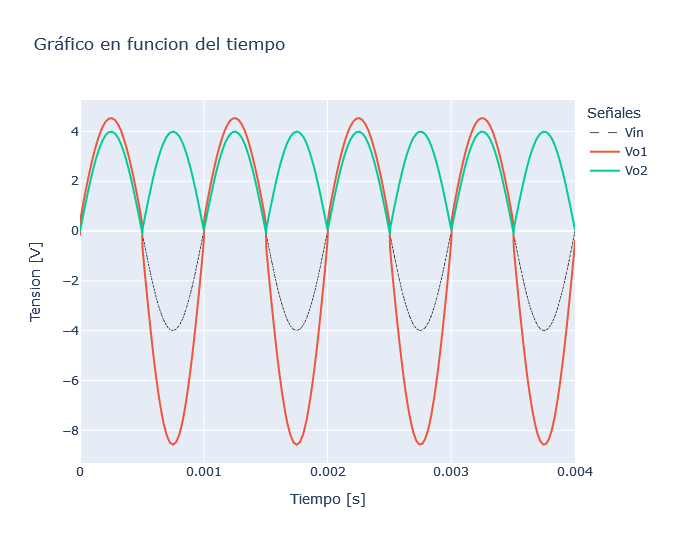
\includegraphics[width=0.9\linewidth]{Secciones/Circuito3/TP1_3_Vo1_Vo2_Vin_vs_t.png}
    \caption{Tensiones de salida del rectificador}
    \label{fig:TP1_3_Vo1_Vo2_Vin_vs_t}
\end{figure}

Para terminar, se graficó la evolución de la amplitud de la señal de salida en función de aquella de la señal de entrada y se observó que la amplitud maxima para una entrada senoidal es de 4 V.

\begin{figure}[H]
    \centering
    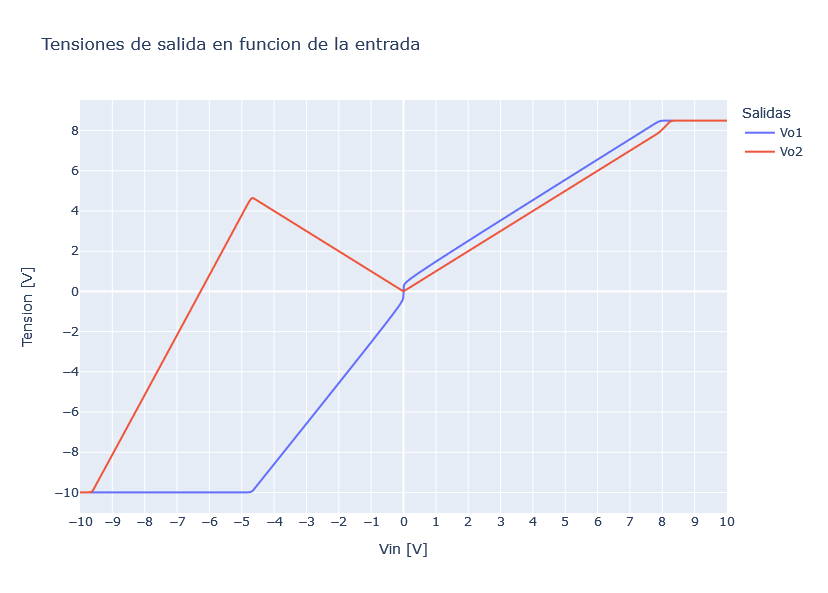
\includegraphics[width=0.9\linewidth]{Secciones/Circuito3/TP1_3_Vo1_Vo2_vs_Vin.png}
    \caption{Simulación entrada/salida del rectificador}
    \label{fig:TP1_3_Vo1_Vo2_vs_Vin}
\end{figure}

\begin{table}[h!]
\centering
\begin{tabular}{|c||c|c|c|}
\hline
\textbf{Vin} & \textbf{Vout 1} & \textbf{Vout 2} \\ \hline
10 mV    & 280 mV  & 9.75 mV  \\ \hline
50 mV   & 394 mV  & 49,7 mV    \\ \hline
100 mV   & 475 mV   & 99,8 mV   \\ \hline
500 mV   & 948 mV & 499 mV  \\ \hline
1 V   & 1,48 V & 1 V  \\ \hline
2 V   & 2,51 V & 2 V    \\ \hline
\end{tabular}
\caption{Tensiones de salida según Vin.}
\label{tab:TP1_3_Vo1_Vo2_vs_Vin}
\end{table}
%\subsection{Experimental}

%En el análisis de modo común:




%\subsection{II.4. Comparación de los resultados teóricos, de simulación y experimentales}

%En la siguiente tabla, reunimos los resultados obtenidos por teoricamente, por simulación y experimentalmente. También calculamos los errores relativos entre los resultados obtenidos experimentalmente con los resultados obtenidos por simulación y teóricamente.
%Para Vin=1V y Vin=3V, los errores relativos entre simulación y teoría son extremadamente pequeños (menor a 1%), como previamente. Para esos valores de Vin, los errores exp/simu y exp/teoría quedan bastante pequeños (con un máximo de 10,4%).
%En contrario, podemos ver que para valores más altos de Vin, los errores son mucho más grandes porque ocurre el fenómeno de saturación o sea que la tensión de salida es físicamente limitada por la tensión de alimentación del operador operacional. El gráfico de la Figura 35 permite una mejor visualización de esas conclusiones.


\subsection{Conclusión}
En este trabajo de laboratorio, pudimos estudiar tres circuitos y observar sus limitaciones al momento de armarlos físicamente.
El primero circuito, amplificador de tensión, solamente permite amplificar con una ganancia experimental de un poco más de 3 en vez de 4 como lo esperábamos según el análisis teórico y la simulación.
El segundo circuito, cuando lo armamos físicamente, tuvo un comportamiento parecido a lo que pudimos observar en la simulación y durante el análisis teórico.
Para terminar, el tercer circuito tuvo resultados parecidos a los obtenidos por simulación y análisis teórico para valores de Vin bajos, pero vimos que si
aumentamos demasiado Vin, el circuito está limitado físicamente por el valor de su alimentación y ocurre la saturación.
\newpage

%Analisis2
\section{Circuito n° 3: Rectificador de precisión }

\subsection{Análisis Teórico}

\begin{figure}[H]
    \centering
    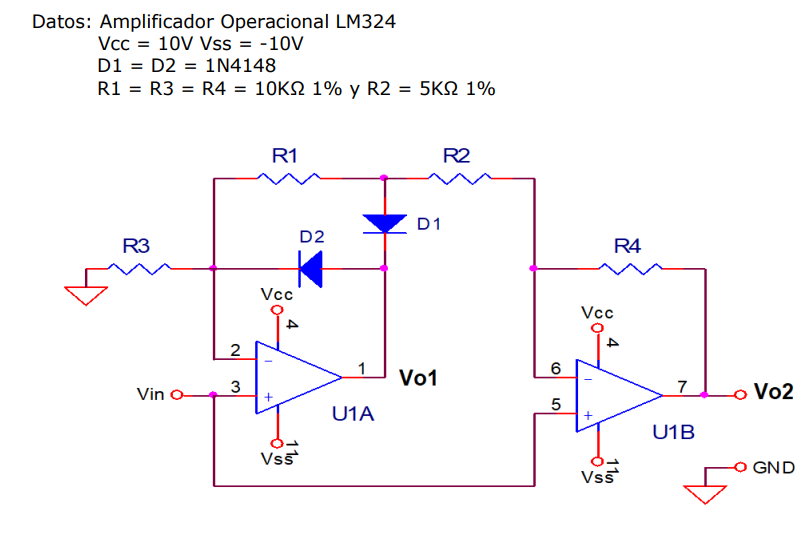
\includegraphics[width=0.5\linewidth]{Secciones/Circuito3/circuito.png}
    \caption{Circuito del rectificador}
    \label{fig:Circuito3}
\end{figure}

Para determinar la tensión de salida Vo en función de la tensión de entrada Vin, se considerarán dos casos: cuando la tensión de entrada es positiva, y cuando la tensión de entrada es negativa.

\[V_0 = f(V_{in}) \ \text{con} \ 0 < V_{in}\]

En estas condiciones, el diodo D2 conduce, mientras que el diodo D1 no, ya que el amplificador U1A se encuentra operando en modo no inversor.
Inicialmente se analizará el caso en que la tensión de entrada del amplificador U1B se encuentra pasivada, entonces la ecuación de corrientes en el nodo ‘6’ resulta:

\begin{equation}
\frac{V_o}{R_4} = \frac{V_in}{R_1 + R_2}
\end{equation}

\begin{equation}
\frac{V_o}{10[k\Omega]} = -\frac{V_{in}}{15[k\Omega]}
\end{equation}

\begin{equation}
V_o = - \frac{2}{3}V_{in}
\end{equation}

Si ahora se pasiva la tensión de entrada del amplificador U1A, se plantea el divisor de tensión en el nodo ‘6’:

\[V_{in} = V_o \frac{R_1+R_2}{R_1+R_2+R_4}\]

\[V_{in} = V_o \frac{15[k\Omega]}{25[k\Omega]}\]

\[V_o = \frac{5}{3}V_{in}\]

Si no se tiene ninguna tensión pasivada, aplicando superposición:

\[V_o = \frac{5}{3}V_{in} - \frac{2}{3}V_{in}\]

\[V_o = V_{in}\]


\subsection{Vo = Vin con 0 \texorpdfstring{$>$}{>} Vin}


En estas nuevas condiciones, el diodo D1 conduce, mientras que el diodo D2 no. Se considerará inicialmente que la tensión a la salida del amplificador U1A se encuentra pasivada. Se plantea el divisor de tensión en el nodo ‘6’:

\[V_{in} = V_o \frac{R_2}{R_2+R_4}\]

\[V_{in} = V_o \frac{5 k\Omega}{15 k\Omega }\]

\[V_o = 3V_{in}\]

Si ahora se considera que la tensión de entrada del amplificador U1B está pasivada, la ecuación de corrientes del nodo ‘6’, tomando VoB como la tensión de salida del amplificador U1B, resulta:

\begin{equation}
\frac{V_{oB}}{R_2} = - \frac{V_o}{R_4}
\end{equation}

\begin{equation}
\frac{V_{oB}}{5 [k\Omega]} = - \frac{V_o}{10 [k\Omega]}
\end{equation}

\begin{equation}
V_o = - 2V_{oB}
\end{equation}

Por otro lado, la tensión de salida VoB se obtiene planteando el divisor de tensión del amplificador U1B:

\[V_{in} = V_{oB} \frac{R_3}{R_1+R_3}\]

\[V_{in} = V_{oB} \frac{10 [k\Omega]}{20 [k\Omega]}\]

\[V_{in} = \frac{1}{2}V_{oB}\]

Reemplazando:

\[V_o = - 4V{in}\]

Si no se tiene ninguna tensión pasivada, aplicando superposición:

\[V_o = 3V{in} - 4V{in}\]

\[V_o = - V{in} \]

En resumen, cuando la tensión de entrada es positiva, la tensión de salida es igual a la tensión de entrada, mientras que cuando la tensión de entrada es negativa, la tensión de salida será positiva y de igual amplitud a la de entrada.


\subsection{Simulación}
Después de encontrar analíticamente la expresión de la tensión de salida en función de aquella de entrada, se simuló el circuito con el software LTSpice. En la figura \ref{fig:TP1_3_Vo1_Vo2_Vin_vs_t}, se visualiza la tensión de salida para una entrada senoidal. 

\begin{figure}[H]
    \centering
    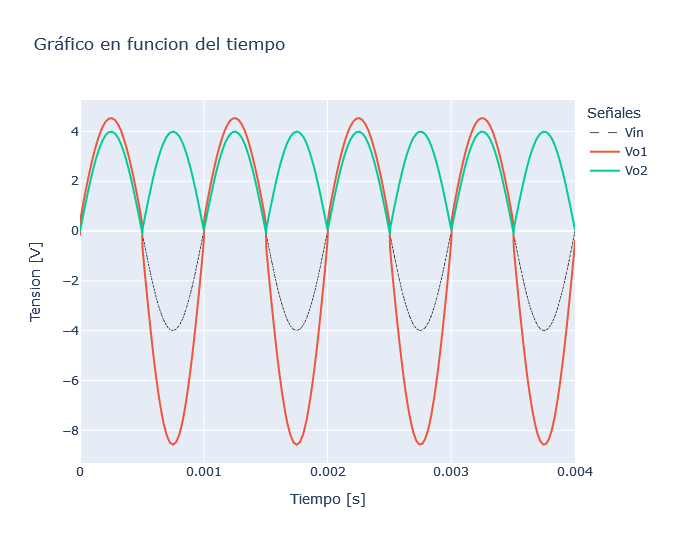
\includegraphics[width=0.9\linewidth]{Secciones/Circuito3/TP1_3_Vo1_Vo2_Vin_vs_t.png}
    \caption{Tensiones de salida del rectificador}
    \label{fig:TP1_3_Vo1_Vo2_Vin_vs_t}
\end{figure}

Para terminar, se graficó la evolución de la amplitud de la señal de salida en función de aquella de la señal de entrada y se observó que la amplitud maxima para una entrada senoidal es de 4 V.

\begin{figure}[H]
    \centering
    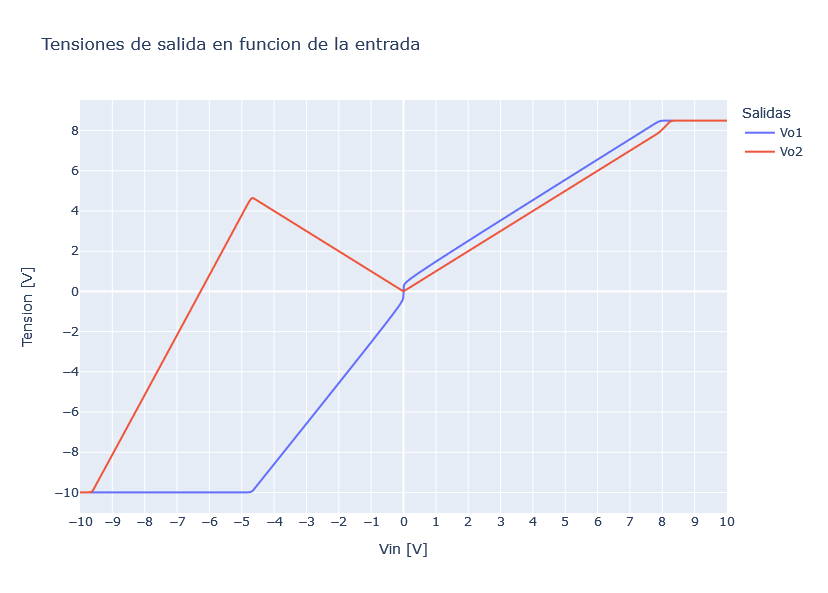
\includegraphics[width=0.9\linewidth]{Secciones/Circuito3/TP1_3_Vo1_Vo2_vs_Vin.png}
    \caption{Simulación entrada/salida del rectificador}
    \label{fig:TP1_3_Vo1_Vo2_vs_Vin}
\end{figure}

\begin{table}[h!]
\centering
\begin{tabular}{|c||c|c|c|}
\hline
\textbf{Vin} & \textbf{Vout 1} & \textbf{Vout 2} \\ \hline
10 mV    & 280 mV  & 9.75 mV  \\ \hline
50 mV   & 394 mV  & 49,7 mV    \\ \hline
100 mV   & 475 mV   & 99,8 mV   \\ \hline
500 mV   & 948 mV & 499 mV  \\ \hline
1 V   & 1,48 V & 1 V  \\ \hline
2 V   & 2,51 V & 2 V    \\ \hline
\end{tabular}
\caption{Tensiones de salida según Vin.}
\label{tab:TP1_3_Vo1_Vo2_vs_Vin}
\end{table}
%\subsection{Experimental}

%En el análisis de modo común:




%\subsection{II.4. Comparación de los resultados teóricos, de simulación y experimentales}

%En la siguiente tabla, reunimos los resultados obtenidos por teoricamente, por simulación y experimentalmente. También calculamos los errores relativos entre los resultados obtenidos experimentalmente con los resultados obtenidos por simulación y teóricamente.
%Para Vin=1V y Vin=3V, los errores relativos entre simulación y teoría son extremadamente pequeños (menor a 1%), como previamente. Para esos valores de Vin, los errores exp/simu y exp/teoría quedan bastante pequeños (con un máximo de 10,4%).
%En contrario, podemos ver que para valores más altos de Vin, los errores son mucho más grandes porque ocurre el fenómeno de saturación o sea que la tensión de salida es físicamente limitada por la tensión de alimentación del operador operacional. El gráfico de la Figura 35 permite una mejor visualización de esas conclusiones.


\subsection{Conclusión}
En este trabajo de laboratorio, pudimos estudiar tres circuitos y observar sus limitaciones al momento de armarlos físicamente.
El primero circuito, amplificador de tensión, solamente permite amplificar con una ganancia experimental de un poco más de 3 en vez de 4 como lo esperábamos según el análisis teórico y la simulación.
El segundo circuito, cuando lo armamos físicamente, tuvo un comportamiento parecido a lo que pudimos observar en la simulación y durante el análisis teórico.
Para terminar, el tercer circuito tuvo resultados parecidos a los obtenidos por simulación y análisis teórico para valores de Vin bajos, pero vimos que si
aumentamos demasiado Vin, el circuito está limitado físicamente por el valor de su alimentación y ocurre la saturación.
\newpage

 \section{Circuito n° 3: Rectificador de precisión }

\subsection{Análisis Teórico}

\begin{figure}[H]
    \centering
    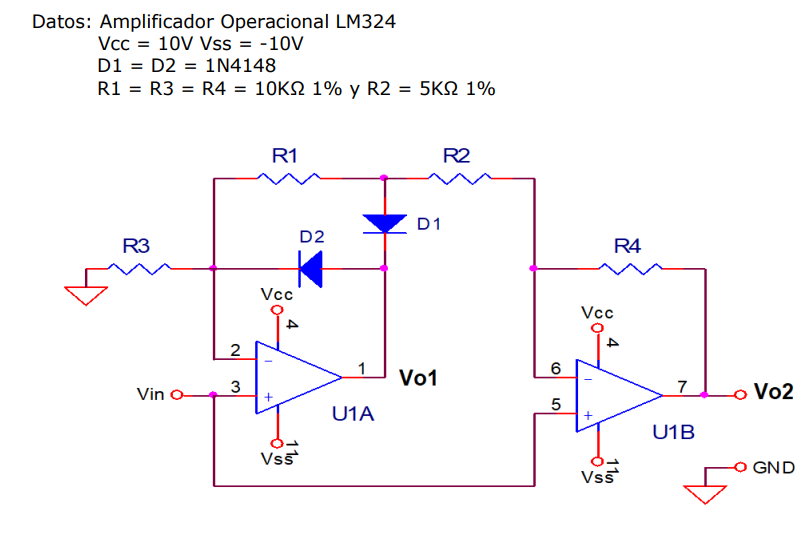
\includegraphics[width=0.5\linewidth]{Secciones/Circuito3/circuito.png}
    \caption{Circuito del rectificador}
    \label{fig:Circuito3}
\end{figure}

Para determinar la tensión de salida Vo en función de la tensión de entrada Vin, se considerarán dos casos: cuando la tensión de entrada es positiva, y cuando la tensión de entrada es negativa.

\[V_0 = f(V_{in}) \ \text{con} \ 0 < V_{in}\]

En estas condiciones, el diodo D2 conduce, mientras que el diodo D1 no, ya que el amplificador U1A se encuentra operando en modo no inversor.
Inicialmente se analizará el caso en que la tensión de entrada del amplificador U1B se encuentra pasivada, entonces la ecuación de corrientes en el nodo ‘6’ resulta:

\begin{equation}
\frac{V_o}{R_4} = \frac{V_in}{R_1 + R_2}
\end{equation}

\begin{equation}
\frac{V_o}{10[k\Omega]} = -\frac{V_{in}}{15[k\Omega]}
\end{equation}

\begin{equation}
V_o = - \frac{2}{3}V_{in}
\end{equation}

Si ahora se pasiva la tensión de entrada del amplificador U1A, se plantea el divisor de tensión en el nodo ‘6’:

\[V_{in} = V_o \frac{R_1+R_2}{R_1+R_2+R_4}\]

\[V_{in} = V_o \frac{15[k\Omega]}{25[k\Omega]}\]

\[V_o = \frac{5}{3}V_{in}\]

Si no se tiene ninguna tensión pasivada, aplicando superposición:

\[V_o = \frac{5}{3}V_{in} - \frac{2}{3}V_{in}\]

\[V_o = V_{in}\]


\subsection{Vo = Vin con 0 \texorpdfstring{$>$}{>} Vin}


En estas nuevas condiciones, el diodo D1 conduce, mientras que el diodo D2 no. Se considerará inicialmente que la tensión a la salida del amplificador U1A se encuentra pasivada. Se plantea el divisor de tensión en el nodo ‘6’:

\[V_{in} = V_o \frac{R_2}{R_2+R_4}\]

\[V_{in} = V_o \frac{5 k\Omega}{15 k\Omega }\]

\[V_o = 3V_{in}\]

Si ahora se considera que la tensión de entrada del amplificador U1B está pasivada, la ecuación de corrientes del nodo ‘6’, tomando VoB como la tensión de salida del amplificador U1B, resulta:

\begin{equation}
\frac{V_{oB}}{R_2} = - \frac{V_o}{R_4}
\end{equation}

\begin{equation}
\frac{V_{oB}}{5 [k\Omega]} = - \frac{V_o}{10 [k\Omega]}
\end{equation}

\begin{equation}
V_o = - 2V_{oB}
\end{equation}

Por otro lado, la tensión de salida VoB se obtiene planteando el divisor de tensión del amplificador U1B:

\[V_{in} = V_{oB} \frac{R_3}{R_1+R_3}\]

\[V_{in} = V_{oB} \frac{10 [k\Omega]}{20 [k\Omega]}\]

\[V_{in} = \frac{1}{2}V_{oB}\]

Reemplazando:

\[V_o = - 4V{in}\]

Si no se tiene ninguna tensión pasivada, aplicando superposición:

\[V_o = 3V{in} - 4V{in}\]

\[V_o = - V{in} \]

En resumen, cuando la tensión de entrada es positiva, la tensión de salida es igual a la tensión de entrada, mientras que cuando la tensión de entrada es negativa, la tensión de salida será positiva y de igual amplitud a la de entrada.


\subsection{Simulación}
Después de encontrar analíticamente la expresión de la tensión de salida en función de aquella de entrada, se simuló el circuito con el software LTSpice. En la figura \ref{fig:TP1_3_Vo1_Vo2_Vin_vs_t}, se visualiza la tensión de salida para una entrada senoidal. 

\begin{figure}[H]
    \centering
    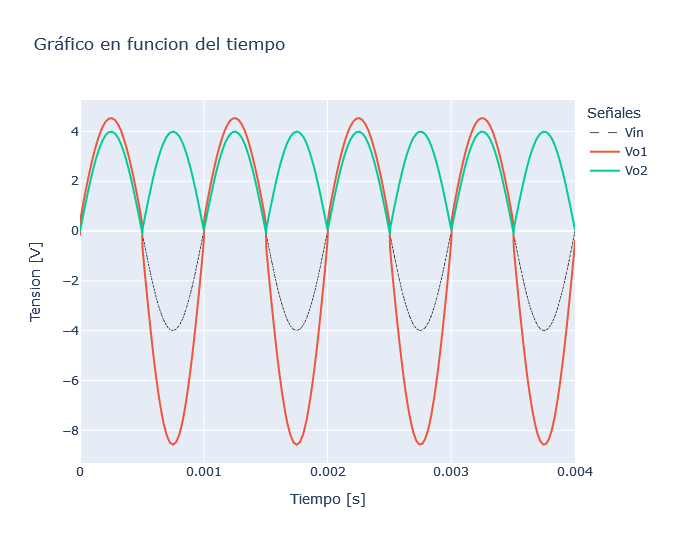
\includegraphics[width=0.9\linewidth]{Secciones/Circuito3/TP1_3_Vo1_Vo2_Vin_vs_t.png}
    \caption{Tensiones de salida del rectificador}
    \label{fig:TP1_3_Vo1_Vo2_Vin_vs_t}
\end{figure}

Para terminar, se graficó la evolución de la amplitud de la señal de salida en función de aquella de la señal de entrada y se observó que la amplitud maxima para una entrada senoidal es de 4 V.

\begin{figure}[H]
    \centering
    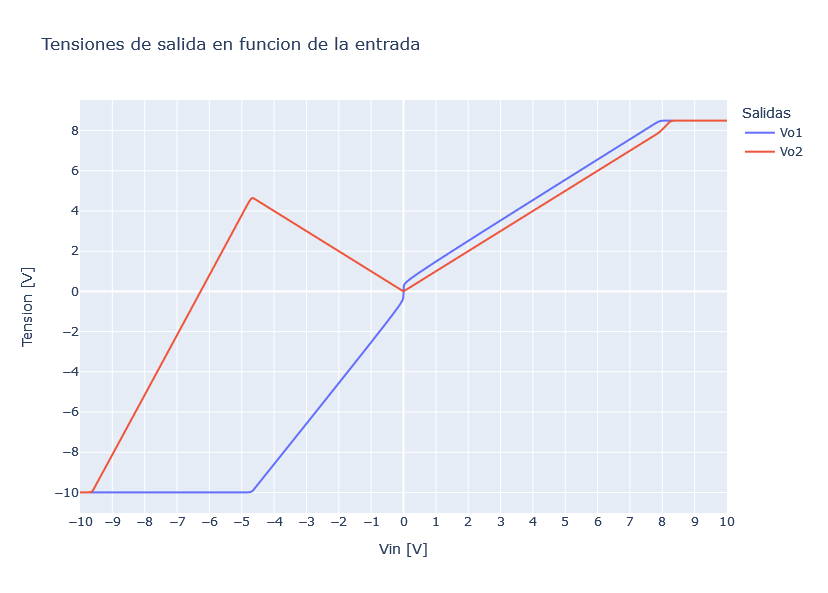
\includegraphics[width=0.9\linewidth]{Secciones/Circuito3/TP1_3_Vo1_Vo2_vs_Vin.png}
    \caption{Simulación entrada/salida del rectificador}
    \label{fig:TP1_3_Vo1_Vo2_vs_Vin}
\end{figure}

\begin{table}[h!]
\centering
\begin{tabular}{|c||c|c|c|}
\hline
\textbf{Vin} & \textbf{Vout 1} & \textbf{Vout 2} \\ \hline
10 mV    & 280 mV  & 9.75 mV  \\ \hline
50 mV   & 394 mV  & 49,7 mV    \\ \hline
100 mV   & 475 mV   & 99,8 mV   \\ \hline
500 mV   & 948 mV & 499 mV  \\ \hline
1 V   & 1,48 V & 1 V  \\ \hline
2 V   & 2,51 V & 2 V    \\ \hline
\end{tabular}
\caption{Tensiones de salida según Vin.}
\label{tab:TP1_3_Vo1_Vo2_vs_Vin}
\end{table}
%\subsection{Experimental}

%En el análisis de modo común:




%\subsection{II.4. Comparación de los resultados teóricos, de simulación y experimentales}

%En la siguiente tabla, reunimos los resultados obtenidos por teoricamente, por simulación y experimentalmente. También calculamos los errores relativos entre los resultados obtenidos experimentalmente con los resultados obtenidos por simulación y teóricamente.
%Para Vin=1V y Vin=3V, los errores relativos entre simulación y teoría son extremadamente pequeños (menor a 1%), como previamente. Para esos valores de Vin, los errores exp/simu y exp/teoría quedan bastante pequeños (con un máximo de 10,4%).
%En contrario, podemos ver que para valores más altos de Vin, los errores son mucho más grandes porque ocurre el fenómeno de saturación o sea que la tensión de salida es físicamente limitada por la tensión de alimentación del operador operacional. El gráfico de la Figura 35 permite una mejor visualización de esas conclusiones.


\subsection{Conclusión}
En este trabajo de laboratorio, pudimos estudiar tres circuitos y observar sus limitaciones al momento de armarlos físicamente.
El primero circuito, amplificador de tensión, solamente permite amplificar con una ganancia experimental de un poco más de 3 en vez de 4 como lo esperábamos según el análisis teórico y la simulación.
El segundo circuito, cuando lo armamos físicamente, tuvo un comportamiento parecido a lo que pudimos observar en la simulación y durante el análisis teórico.
Para terminar, el tercer circuito tuvo resultados parecidos a los obtenidos por simulación y análisis teórico para valores de Vin bajos, pero vimos que si
aumentamos demasiado Vin, el circuito está limitado físicamente por el valor de su alimentación y ocurre la saturación.
\newpage

\section{Circuito n° 3: Rectificador de precisión }

\subsection{Análisis Teórico}

\begin{figure}[H]
    \centering
    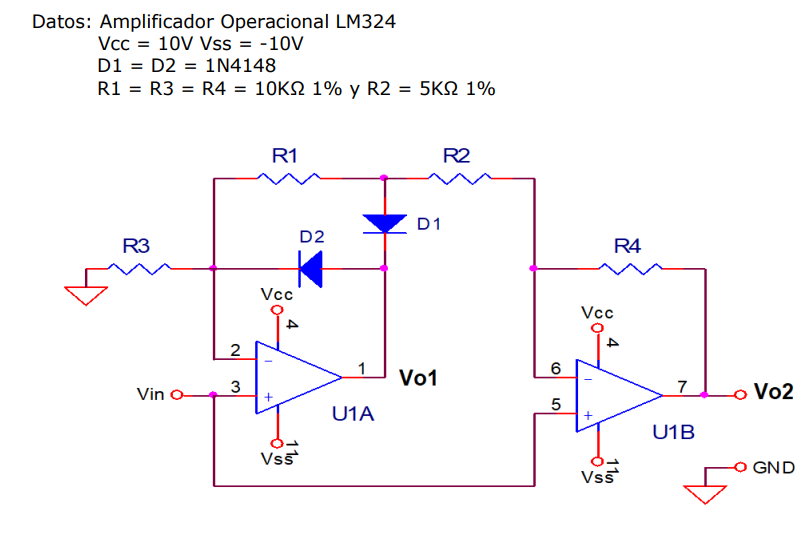
\includegraphics[width=0.5\linewidth]{Secciones/Circuito3/circuito.png}
    \caption{Circuito del rectificador}
    \label{fig:Circuito3}
\end{figure}

Para determinar la tensión de salida Vo en función de la tensión de entrada Vin, se considerarán dos casos: cuando la tensión de entrada es positiva, y cuando la tensión de entrada es negativa.

\[V_0 = f(V_{in}) \ \text{con} \ 0 < V_{in}\]

En estas condiciones, el diodo D2 conduce, mientras que el diodo D1 no, ya que el amplificador U1A se encuentra operando en modo no inversor.
Inicialmente se analizará el caso en que la tensión de entrada del amplificador U1B se encuentra pasivada, entonces la ecuación de corrientes en el nodo ‘6’ resulta:

\begin{equation}
\frac{V_o}{R_4} = \frac{V_in}{R_1 + R_2}
\end{equation}

\begin{equation}
\frac{V_o}{10[k\Omega]} = -\frac{V_{in}}{15[k\Omega]}
\end{equation}

\begin{equation}
V_o = - \frac{2}{3}V_{in}
\end{equation}

Si ahora se pasiva la tensión de entrada del amplificador U1A, se plantea el divisor de tensión en el nodo ‘6’:

\[V_{in} = V_o \frac{R_1+R_2}{R_1+R_2+R_4}\]

\[V_{in} = V_o \frac{15[k\Omega]}{25[k\Omega]}\]

\[V_o = \frac{5}{3}V_{in}\]

Si no se tiene ninguna tensión pasivada, aplicando superposición:

\[V_o = \frac{5}{3}V_{in} - \frac{2}{3}V_{in}\]

\[V_o = V_{in}\]


\subsection{Vo = Vin con 0 \texorpdfstring{$>$}{>} Vin}


En estas nuevas condiciones, el diodo D1 conduce, mientras que el diodo D2 no. Se considerará inicialmente que la tensión a la salida del amplificador U1A se encuentra pasivada. Se plantea el divisor de tensión en el nodo ‘6’:

\[V_{in} = V_o \frac{R_2}{R_2+R_4}\]

\[V_{in} = V_o \frac{5 k\Omega}{15 k\Omega }\]

\[V_o = 3V_{in}\]

Si ahora se considera que la tensión de entrada del amplificador U1B está pasivada, la ecuación de corrientes del nodo ‘6’, tomando VoB como la tensión de salida del amplificador U1B, resulta:

\begin{equation}
\frac{V_{oB}}{R_2} = - \frac{V_o}{R_4}
\end{equation}

\begin{equation}
\frac{V_{oB}}{5 [k\Omega]} = - \frac{V_o}{10 [k\Omega]}
\end{equation}

\begin{equation}
V_o = - 2V_{oB}
\end{equation}

Por otro lado, la tensión de salida VoB se obtiene planteando el divisor de tensión del amplificador U1B:

\[V_{in} = V_{oB} \frac{R_3}{R_1+R_3}\]

\[V_{in} = V_{oB} \frac{10 [k\Omega]}{20 [k\Omega]}\]

\[V_{in} = \frac{1}{2}V_{oB}\]

Reemplazando:

\[V_o = - 4V{in}\]

Si no se tiene ninguna tensión pasivada, aplicando superposición:

\[V_o = 3V{in} - 4V{in}\]

\[V_o = - V{in} \]

En resumen, cuando la tensión de entrada es positiva, la tensión de salida es igual a la tensión de entrada, mientras que cuando la tensión de entrada es negativa, la tensión de salida será positiva y de igual amplitud a la de entrada.


\subsection{Simulación}
Después de encontrar analíticamente la expresión de la tensión de salida en función de aquella de entrada, se simuló el circuito con el software LTSpice. En la figura \ref{fig:TP1_3_Vo1_Vo2_Vin_vs_t}, se visualiza la tensión de salida para una entrada senoidal. 

\begin{figure}[H]
    \centering
    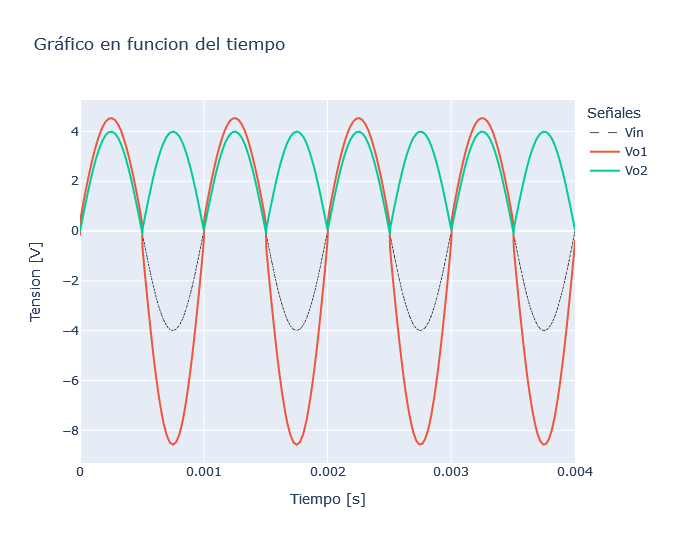
\includegraphics[width=0.9\linewidth]{Secciones/Circuito3/TP1_3_Vo1_Vo2_Vin_vs_t.png}
    \caption{Tensiones de salida del rectificador}
    \label{fig:TP1_3_Vo1_Vo2_Vin_vs_t}
\end{figure}

Para terminar, se graficó la evolución de la amplitud de la señal de salida en función de aquella de la señal de entrada y se observó que la amplitud maxima para una entrada senoidal es de 4 V.

\begin{figure}[H]
    \centering
    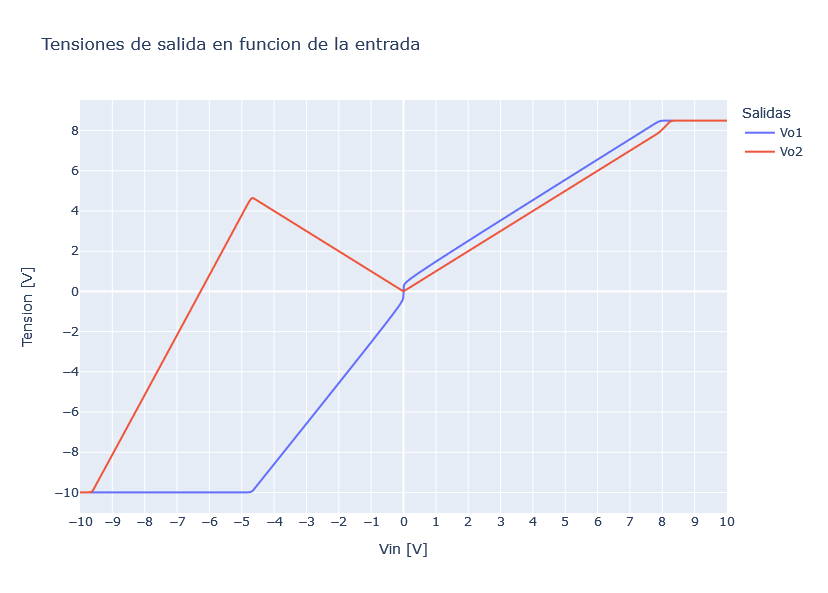
\includegraphics[width=0.9\linewidth]{Secciones/Circuito3/TP1_3_Vo1_Vo2_vs_Vin.png}
    \caption{Simulación entrada/salida del rectificador}
    \label{fig:TP1_3_Vo1_Vo2_vs_Vin}
\end{figure}

\begin{table}[h!]
\centering
\begin{tabular}{|c||c|c|c|}
\hline
\textbf{Vin} & \textbf{Vout 1} & \textbf{Vout 2} \\ \hline
10 mV    & 280 mV  & 9.75 mV  \\ \hline
50 mV   & 394 mV  & 49,7 mV    \\ \hline
100 mV   & 475 mV   & 99,8 mV   \\ \hline
500 mV   & 948 mV & 499 mV  \\ \hline
1 V   & 1,48 V & 1 V  \\ \hline
2 V   & 2,51 V & 2 V    \\ \hline
\end{tabular}
\caption{Tensiones de salida según Vin.}
\label{tab:TP1_3_Vo1_Vo2_vs_Vin}
\end{table}
%\subsection{Experimental}

%En el análisis de modo común:




%\subsection{II.4. Comparación de los resultados teóricos, de simulación y experimentales}

%En la siguiente tabla, reunimos los resultados obtenidos por teoricamente, por simulación y experimentalmente. También calculamos los errores relativos entre los resultados obtenidos experimentalmente con los resultados obtenidos por simulación y teóricamente.
%Para Vin=1V y Vin=3V, los errores relativos entre simulación y teoría son extremadamente pequeños (menor a 1%), como previamente. Para esos valores de Vin, los errores exp/simu y exp/teoría quedan bastante pequeños (con un máximo de 10,4%).
%En contrario, podemos ver que para valores más altos de Vin, los errores son mucho más grandes porque ocurre el fenómeno de saturación o sea que la tensión de salida es físicamente limitada por la tensión de alimentación del operador operacional. El gráfico de la Figura 35 permite una mejor visualización de esas conclusiones.


\subsection{Conclusión}
En este trabajo de laboratorio, pudimos estudiar tres circuitos y observar sus limitaciones al momento de armarlos físicamente.
El primero circuito, amplificador de tensión, solamente permite amplificar con una ganancia experimental de un poco más de 3 en vez de 4 como lo esperábamos según el análisis teórico y la simulación.
El segundo circuito, cuando lo armamos físicamente, tuvo un comportamiento parecido a lo que pudimos observar en la simulación y durante el análisis teórico.
Para terminar, el tercer circuito tuvo resultados parecidos a los obtenidos por simulación y análisis teórico para valores de Vin bajos, pero vimos que si
aumentamos demasiado Vin, el circuito está limitado físicamente por el valor de su alimentación y ocurre la saturación.
\newpage

\section{Conclusión}
En este trabajo de laboratorio, se lograron estudiar cuatro circuitos y observar sus limitaciones al momento de armarlos físicamente.

El primer circuito, amplificador diferencial, solamente permite amplificar con una ganancia diferencial de un poco más de 3 veces en lugar de 4 veces como lo esperábamos según el análisis teórico y la simulación. El segundo circuito se comportó muy similar al caso estudiado en la simulación y en el análisis teórico del mismo. El tercer circuito se asemejaba al simulado y se comportaba según el análisis teórico planteado para valores de tensión de entrada bajos. Al aumentar demasiado la tensión de entrada, el circuito se vio limitado físicamente por el valor de su alimentación y pasó a saturación. Además, se logró verificar tanto por simulaciones como por mediciones en el laboratorio los efectos que traen la no linealidad de los componentes. El último circuito armado funcionó de manera correcta al armarlo físicamente hasta que se trabajó con alimentación asimétrica; a partir de este momento se encontraron diferencias notables entre el modelo simulado y lo medido.


\printbibliography

\end{document}
